%!TEX root=../book.tex

\chapter[Research Design]{Research Design}
\section{Relating Design and Analysis}

\subsection{Garbage In, Garbage Out}
This is a book about applied statistical analysis. So why are we including a whole chapter on considerations for designing your experiments?

It's simple: if your experimental design is bad, or your data collection methods are bad, then your results will be bad. Choosing an appropriate statistical analysis, although that's the crux of this book, does not guarantee that you will walk away with interpretable, generalizable results. For that, you need a well-designed experiment.

One of the biggest reasons that experiments are ever conducted is to evidence (or at least plausibly suggest) a causal link between one or more variables and a particular outcome. To do this, we design experiments with various control and experimental groups, all of which we assume are \textbf{probabilistically equivalent}. This means that we know the probability of finding a difference between any of our groups on the basis of pure chance alone. That is, this allows us to believe that just because we find a difference between two groups on one variable, we cannot infer anything about differences among other variables. In turn, this (1) assures us that our findings are due to differences in the treatment and not in the participants and (2) lets us generalize our results to larger populations.

However, to do this, we need to ensure that our studies are both internally and externally valid. \textbf{Internal validity} refers to our ability to justify our conclusions: it is what enables a researcher to establish a causal link between a treatment and an effect. \textbf{External validity} is an extension of this: it is our ability to take our causal inferences and apply them to populations (rather than only to the sample used in a study).

\subsection{Accuracy and Precision}

In research, both accuracy\index{Accuracy} and precision\index{Precision} are a concern to the researcher: accuracy being how well you are measuring what you actually are trying to measure and precision being how often you measure that trait. Let's take the example of a game of darts: your accuracy is how close to the bullseye you are on any given throw; your precision is how much your aim varies throw-to-throw (Figure \ref{fig:research01}).

Another way of phrasing this is that your accuracy is how far away you are from something's true value and your precision is how reproducible your measurement is. When talking about research, accuracy translates to \textbf{validity}\index{Validity} and precision\index{Precision} translates to \textbf{reliability}.

Understandably, both are important to good research; however, we will only focus on validity in this chapter. Measures of reliability differ widely discipline-to-discipline and a discussion of inter-rater reliability isn't going to translate into the context of a physics experiment. If you have questions about reliability, talk to others in your field of study or search around on the internet!

\begin{figure*}[htp]
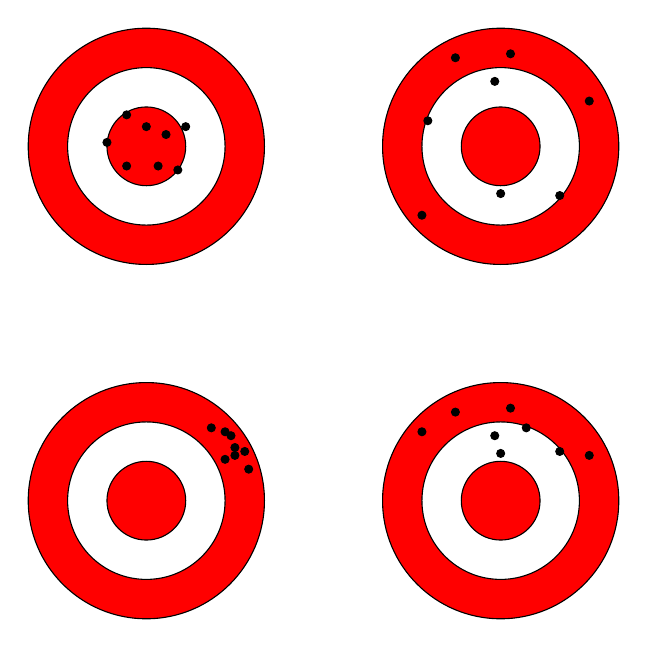
\begin{tikzpicture}[>=latex]
% Upper Left
% Accurate and precise
% Concentric circles and radius labels
  \filldraw[fill=red] (0,0) circle (1.5);
  \filldraw[fill=white] (0,0) circle (1);
  \filldraw[fill=red] (0,0) circle (.5);
  
  \filldraw[fill=black] (.5,.25) circle (.05);
  \filldraw[fill=black] (.25,.15) circle (.05);
  \filldraw[fill=black] (0,.25) circle (.05);
  \filldraw[fill=black] (.15,-.25) circle (.05);
  \filldraw[fill=black] (-.5,.05) circle (.05);
  \filldraw[fill=black] (-.25,-.25) circle (.05);
  \filldraw[fill=black] (-.25,.4) circle (.05);
  \filldraw[fill=black] (.4,-.3) circle (.05);

% Lower Left
% Precise, not accurate
% Concentric circles and radius labels
\begin{scope}[yshift=-4.5cm]
  \filldraw[fill=red] (0,0) circle (1.5);
  \filldraw[fill=white] (0,0) circle (1);
  \filldraw[fill=red] (0,0) circle (0.5);
  
  \filldraw[fill=black] (1.25,0.625) circle (0.05);
  \filldraw[fill=black] (1.125,0.575) circle (0.05);
  \filldraw[fill=black] (1,0.875) circle (0.05);
  \filldraw[fill=black] (1,0.525) circle (0.05);
  \filldraw[fill=black] (1.3,.4) circle (0.05);
  \filldraw[fill=black] (1.075,0.825) circle (0.05);
  \filldraw[fill=black] (0.825,0.925) circle (0.05);
  \filldraw[fill=black] (1.125,0.675) circle (0.05);
\end{scope}

% Upper Right
% Accurate, not precise
% Concentric circles and radius labels
\begin{scope}[xshift=4.5cm]
  \filldraw[fill=red] (0,0) circle (1.5);
  \filldraw[fill=white] (0,0) circle (1);
  \filldraw[fill=red] (0,0) circle (0.5);
  
	\filldraw[fill=black] (0.75, -0.625) circle (0.05);
	\filldraw[fill=black] (1.125, 0.575) circle (0.05);
	\filldraw[fill=black] (-1, -0.875) circle (0.05);
	\filldraw[fill=black] (-0.575, 1.125) circle (0.05);
	\filldraw[fill=black] (0, -0.6) circle (0.05);
	\filldraw[fill=black] (-0.075, 0.825) circle (0.05);
	\filldraw[fill=black] (-0.925, 0.325) circle (0.05);
	\filldraw[fill=black] (0.125, 1.175) circle (0.05);
\end{scope}

% Lower Right
% Inaccurate and imprecise
% Concentric circles and radius labels
\begin{scope}[yshift=-4.5cm, xshift=4.5cm]
  \filldraw[fill=red] (0,0) circle (1.5);
  \filldraw[fill=white] (0,0) circle (1);
  \filldraw[fill=red] (0,0) circle (0.5);
  
	\filldraw[fill=black] (0.75, 0.625) circle (0.05);
	\filldraw[fill=black] (1.125, 0.575) circle (0.05);
	\filldraw[fill=black] (-1, 0.875) circle (0.05);
	\filldraw[fill=black] (-0.575, 1.125) circle (0.05);
	\filldraw[fill=black] (0, 0.6) circle (0.05);
	\filldraw[fill=black] (-0.075, 0.825) circle (0.05);
	\filldraw[fill=black] (0.325, 0.925) circle (0.05);
	\filldraw[fill=black] (0.125, 1.175) circle (0.05);
\end{scope}
\end{tikzpicture}
\caption{Accuracy and precision in a game of darts. High accuracy and high precision (upper left); high accuracy and low precision (upper right); low accuracy and high precision (lower left); low accuracy and low precision (lower right). NOTE: The upper right circle is ``accurate'' because each of the darts \textbf{averages out} to near the bullseye.}
\label{fig:research01}
\end{figure*}

\section{Designing Sound Experiments}

\subsection{Internal Validity}
Again, \textbf{internal validity}\index{Internal validity} reflects the ability of a researcher to draw causal conclusions from a study. Generally, for a study to be internally valid, it must broadly satisfy three conditions:

\begin{enumerate}
  \item Temporal precedence (the cause precedes the effect);
  \item Covariation (the cause and effect are related); and
  \item Nonspuriousness (there are no other plausible explanations for the observed effect).
\end{enumerate}

Unfortunately, there are a number of practices that can threaten a study's internal validity. A short list of these is included below.

\subsubsection{Confounding}
A confounding variable is one that is not controlled for by the experimenter, yet that correlates with both the dependent and independent variables. This may result in the appearance of a relationship between the two variables when in actuality neither impacts the other, but both are mediated by a third variable. This is termed a \textbf{spurious relationship}. For instance, if we look at U.S. spending on science and technology and the number of suicides by hanging, strangulation, and suffocation from 1999 through 2009 we see that they correlate (Figure \ref{fig:research02}). And pretty highly. 

\begin{figure}[htp]
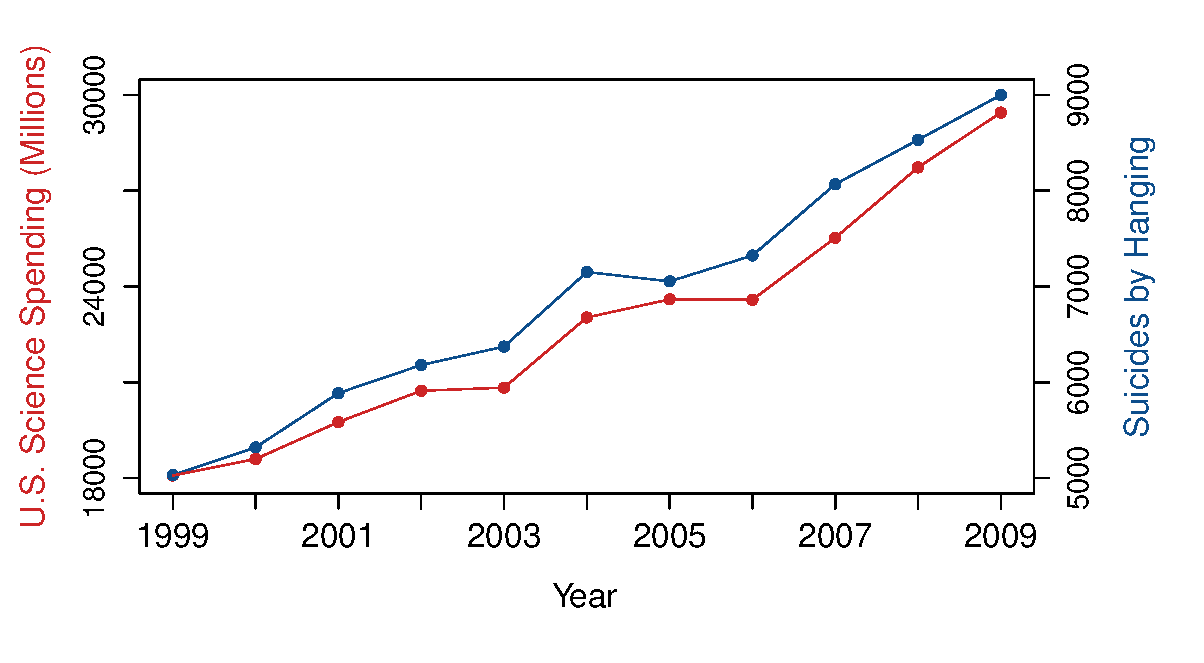
\includegraphics[width=\textwidth]{research01}
\caption{Correlation between U.S. spending on science and suicides by hanging}
\label{fig:research02}
\end{figure}

But that's also an idiotic relationship: U.S. spending on science and technology has no effect on the number of suicides by hanging each year. The fact that these two variables correlate is either purely coincidental or mediated by some third variable that we haven't considered. (For instance, over that 10-year span, the U.S. has experienced both inflation---about 28\%---and population growth---about 13\%---that would each cause the increases that we see in our two variables.)

Yet, if we ignore the absurdity of it and only look at the statistics, we see that there is a highly significant correlation between the two (r = 0.99; t = 23.90; \textit{p}-value $<$ 0.001). That's probably the best correlation (or at least the highest Pearson's r) you'll see in your natural-born life. Without context, that would be a highly convincing correlation. Yet, as soon as we stop and think about this, it becomes clear that this is likely a spurious relationship.

Unfortunately, in many cases, spurious relationships will not be so obvious. As such, the researcher must be careful to randomly select his or her study participants and to carefully control for the manipulated factors in the study to prevent the influence of uncontrolled factors.

\subsubsection{Selection Bias}\index{Sampling strategies}
Selection bias is likely one of the more (if not the most) common threats to the internal validity of a study. The idea here is that the sample of participants is not truly a random and representative sample. (I.e., not every possible participant has an equal chance of being selected for the study and certain groups will be overrepresented while other groups may not be represented at all.) Two common practices that create this type of bias are convenience sampling and voluntary response sampling.

\textbf{Convenience sampling} refers to the practice of only using as your sample pool participants who are easy to reach; \textbf{voluntary response sampling} allows participants to opt in to your study. Unfortunately, these both may skew results, and yet are also common practices in many of the social sciences. Take a psychological experiment, for example: we allow convenience sampling by drawing from the pool of students currently enrolled in an introductory psych course. This pool of participants is neither representative of the university as a whole, nor necessarily generalizable across other universities or to the national population as a whole. Further, these students are usually allowed to choose the studies in which they would like to participate, resulting in voluntary response sampling.

Although neither is necessarily enough to skew the results of a study to the point of it being flatly wrong, considerations such as these do limit the generalizability of one's study. (We'll discuss this more in depth below under the \textbf{Sample Limitations} heading.)

When conducting a study, there are various strategies that you can use to help ensure a representative sample is chosen. A brief list of these includes:

\begin{enumerate}
  \item \textbf{Simple Random Sampling} --- This implies that everyone in a population has an equal probability of being selected. For instance, say that we want to choose 100 students out of a university with 2000 students. A way to simple randomly sample these students would be to put every student's name into a hat and draw 100 names at random without replacements (i.e., not putting a name back into the hat after it has been drawn). This would give any individual student a 1-in-20 (5\%) chance of being selected.
  \item \textbf{Systematic Sampling} --- If you're familiar with Latin, you'll recognize that the English word ``decimate'' derives from the Latin ``decimus'' (meaning ``tenth''). Originally, this referred to the practice of killing every tenth soldier in a mutinous legion. (Happy, right?) Systematic sampling is similar: given a pool of applicants of size \( N \), and knowing that you want \( n \) participants in your study, you choose every \(k^{th} \) individual from the pool where \(k=\frac{N}{n}\). So if we wanted 20 subjects out of a pool of 600, we would arrange them all into a list and pick every 30$^{th}$ person (\(\frac{600}{20}\)) on that list.
  \item \textbf{Stratified Random Sampling} --- Simplifying the actual selection strategies a bit, a stratified random sample is composed of a random sample of participants from different strata of a population (e.g., age group; ethnicity; etc.). Each stratum should be mutually-exclusive (i.e., no individual should be in multiple strata).
  \item \textbf{Cluster Sampling} --- Here, the total population is divided into \href{http://en.wikipedia.org/wiki/Data_clustering}{clusters}. A simple random sample of these groups is selected and from these groups a simple random sample of participants is selected.
\end{enumerate}

\subsubsection{History}
Unfortunately, history is one of the few threats to internal validity that researchers cannot always control for. Occasionally, events outside the scope of an experiment may impact participants' responses to the experiment. (For example, Americans' attitudes to U.S. clandestine operations would probably have differed dramatically if a researcher asked immediately before 9/11 versus immediately after, regardless of the experimental manipulation.)

\subsubsection{Maturation/Mortality}
In longer-term studies, participants may change significantly between measurements (e.g., the concentration of children at 4 years versus 5 years old). Additionally, participants may (and likely will) drop out of longitudinal studies. This is unavoidable; however, should be an important factor for a researcher conducting this type of study to consider and attempt to control for.

\subsubsection{Testing Effects}
When participants are given the same (or a similar) test at multiple points in time (e.g., pretesting and post-testing), participant responses on later tests may change as a function of having been already exposed to the measure. For instance, participants may remember questions and their correct answers; they may know what a ``good'' or ``bad'' response is; etc. In some cases, steps can be taken to identify whether testing effects have biased participant responses (such as a \href{http://www.bing.com/search?q=solomon+four-group+design}{Solomon four-group design}).

\subsubsection{Experimenter bias}
As must as experimenters wish to be objective, we do all have some hypothesis or other that we want to see confirmed or refuted. These personal biases may affect the way in which we interact with participants in experimental and control groups, and by doing so bias their responses or our interpretation of their responses. In many cases this can be eliminated by automating the testing and scoring process and by conducting double-blind experiments in which neither the participant nor the researcher knows which testing group the participant is in.

\subsection{External Validity}\index{External validity}

Given that we can draw causal inferences from our research, we may also want to generalize those results to broader populations. However, researchers often use very specialized populations (college students; psychiatric populations; etc.) that may not be representative of larger groups, or may only be generalizable to \textit{certain} groups, but not to others. For instance, a study that uses a questionnaire based on cultural norms in the US is probably not going to give the same results if it's administered in, say, Finland.

\subsubsection{Treatment Interactions}
Occasionally, an experimental effect may only be observed when multiple treatments interact, or when a treatment interacts with a non-experimental variable such as setting or participant selection. Perhaps the effect only exists in a certain physical location or in an experimental setting (and not in everyday life).

\subsubsection{Order Effects}
In addition to randomizing the selection of participants, researchers should be careful, when possible, to randomize the order of treatment. Specifically, if a participant receives Treatment A and then Treatment B, her response may be different than it would have been had she received Treatment B before Treatment A. By randomizing the treatment order, researchers are able to control for this.

\subsubsection{Hawthorne Effect}
Also known as the observer effect, this is a phenomenon by which individuals act differently while being observed than they would otherwise. (For instance, it probably takes you longer to finish your business in a public restroom than it does at home. That's the Hawthorne effect in action!)

\subsubsection{Rosenthal Effect}
Similar to the Hawthorne Effect, this refers to a tendency for individuals to perform better the more expectation is placed on them to succeed.

\subsubsection{Sample Limitations}
This may refer both to the size and makeup of a researcher's sample. If the number of participants is too small, there is greater risk of sampling error and selecting a non-representative sample from the available pool of participants. Alternately, the participants' intrinsic characteristics (e.g., age, sex, race, education, etc.) may not be representative of the population that a researcher is attempting to study and to reach general conclusions about.

\section{Drawing Conclusions}

The purpose of conducting any experiment is to obtain some ultimate takeaway---an answer to a research question; the creation of new hypotheses and research questions; etc. Being able to do this relies on both a sound experimental design and sound statistical analysis of the data generated by that experiment.

However, what the researcher then does with all that information is just as crucial. It's incredibly easy to do all the right things designing your experiment, conduct all the appropriate statistical tests, and then completely misrepresent the data in your results and discussion. This gets into issues of \textit{p}-hacking, of general statistical literacy, and just the plain old conflict between what the data say and what your research program expects to see.

In academic research, this is one of the problems that I see the most frequently: purported results that don't match up with the statistics presented. And unfortunately, that's one of the things books like this are unable to do a good job teaching: even with sound analytic strategies, it's easy to take any statistically significant result as confirmation of your initial hypotheses, even if the two aren't logically connected. It's this part of the research process where the onus really does fall on the researcher to be diligent and ensure that the claims being made are those that are fully supported by the statistics presented.